\documentclass{article}
\usepackage[T1]{fontenc}
\usepackage{lmodern}
\usepackage{graphicx}
\usepackage{amsmath,amssymb}
\usepackage[a4paper,margin=2cm]{geometry}
\usepackage[absolute,overlay]{textpos}
\setlength{\TPHorizModule}{1mm}
\setlength{\TPVertModule}{1mm}
\usepackage[indonesian]{babel}
\usepackage{hyperref}
\setlength{\emergencystretch}{2em}
% unit: Halaman 12

\begin{document}

% === Halaman 12 (llm) ===

\begin{center}
\textbf{Caesar Cipher Wheel}
\end{center}

\vspace{10mm}

\begin{center}
Enter the key: \textbf{5}
\end{center}

% deskripsi: Ilustrasi interaktif Caesar Cipher Wheel yang menunjukkan dua lingkaran alfabet konsentris untuk enkripsi dan dekripsi teks dengan kunci tertentu.
% bbox normalisasi: [0.3180, 0.2040, 0.6820, 0.8750]
\begin{textblock*}{76.44mm}(66.78mm,60.59mm)
\noindent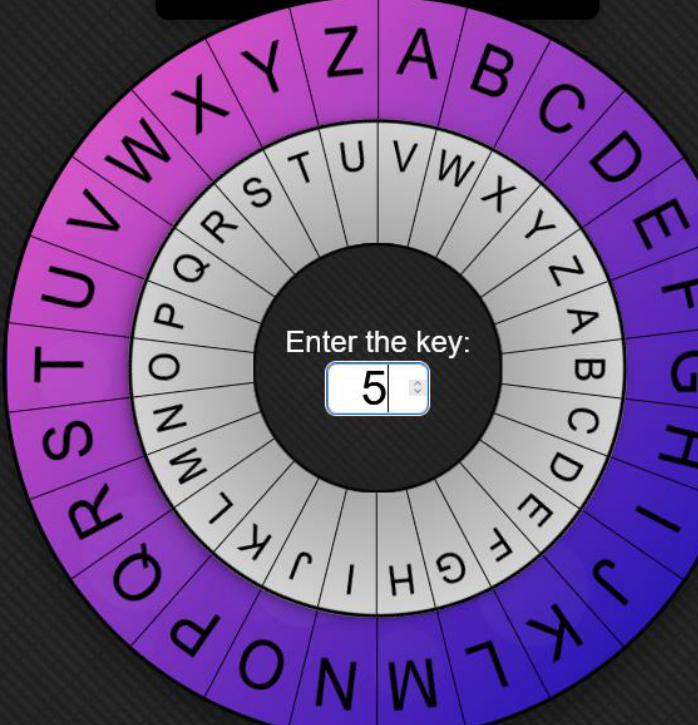
\includegraphics[width=76.44mm,height=199.29mm]{../../images/llm/page_012_img_01.png}%
\end{textblock*}

\end{document}
